\chapteropen{Chapter 8: Agile, XP and Scrum}{chapter-8}
\markboth{Ch. 8 | Agile and Scrum}{}


\begin{studycolumns}
\vspace{0pt}
\begin{eli5box}
A sprint is a short team promise to produce a usable increment and learn from it. The backlog is the prioritised queue; the Product Owner orders value; developers choose and organise feasible work; the Scrum Master helps the process work. Velocity is the team's measured delivery pace, not a demand to work faster.
\end{eli5box}
\textbf{Answer check:} Use the Sprint Goal, actual capacity and completed velocity. Developers retain ownership; the Scrum Master facilitates. Negotiate scope transparently instead of extending the timebox or lowering quality. Incomplete items earn no completed velocity.
\end{studycolumns}

\subsection*{Visual: follow one sprint through its feedback loops}
\sectionlabel{h-visual-follow-one-sprint-through-its-feedback-loops}


\par\smallskip\noindent\begin{minipage}{\linewidth}\centering
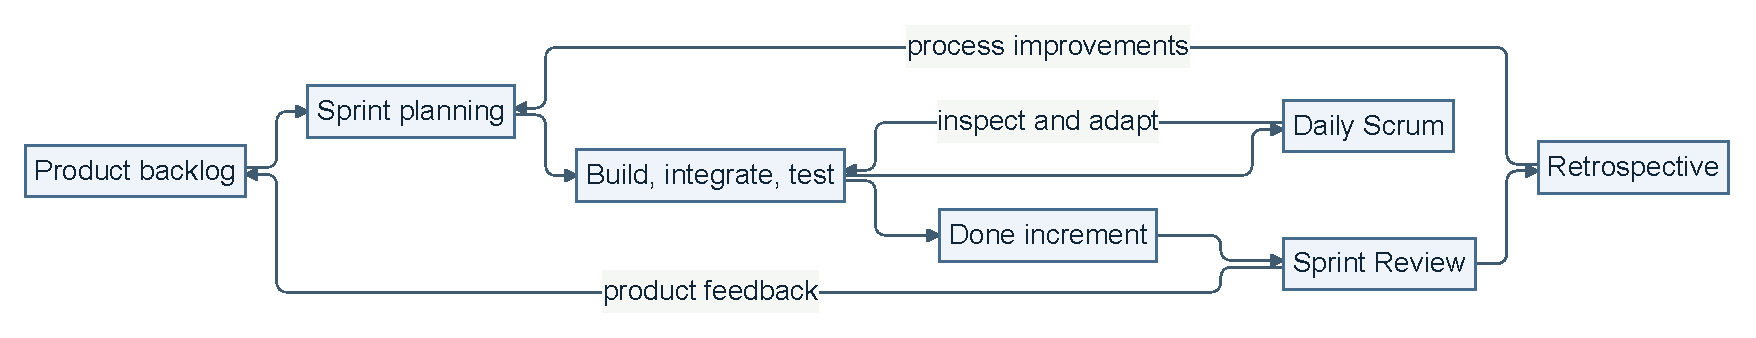
\includegraphics[width=514.00pt]{images/fig-023.pdf}
\captionof{figure}{follow one sprint through its feedback loops}\end{minipage}\par\smallskip

\begin{studycolumns}
\vspace{0pt}



\needspace{4\baselineskip}
\subsection*{8.1 Why agile emerged}
\sectionlabel{h-81-why-agile-emerged}
Rapid delivery became the dominant requirement: requirements change too fast for stable specs; plan-driven development does not meet these needs; agile methods (late 1990s) aimed to \textbf{radically reduce delivery time for working software}.

Agile development characteristics:

\begin{itemize}
\item program specification, design and implementation are \textbf{inter-leaved};
\item the system is developed as \textbf{a series of versions/\allowbreak{}increments}, with stakeholders involved in specification and evaluation of each version;
\item \textbf{frequent delivery} of new versions for evaluation;
\item \textbf{extensive tool support} (e.g. automated testing);
\item \textbf{minimal documentation} --- focus on working code.
\end{itemize}
\needspace{4\baselineskip}
\subsection*{8.2 Agile manifesto (4 values --- quote them exactly)}
\sectionlabel{h-82-agile-manifesto-4-values--quote-them-exactly}

\begin{quote}\small\color{navy}
We are uncovering better ways of developing software by doing it and helping others do it. Through this work we have come to value:

\begin{itemize}
\item \textbf{Individuals and interactions} over processes and tools
\item \textbf{Working software} over comprehensive documentation
\item \textbf{Customer collaboration} over contract negotiation
\item \textbf{Responding to change} over following a plan
\end{itemize}
That is, while there is value in the items on the right, we value the items on the left more.

\end{quote}
\textbf{Trap:} it does \textbf{not} say "no documentation". Both sides have value; the left is \emph{valued more}. Saying "agile means no documentation" is inconsistent with the manifesto.

\needspace{4\baselineskip}
\subsection*{8.3 The five agile principles}
\sectionlabel{h-83-the-five-agile-principles}

\begin{referenceentries}
\textit{\textbf{Principle} / \textbf{Description}}\par\smallskip
\noindent \textbf{\textbf{Customer involvement}}: Customers closely involved throughout; provide and prioritise requirements, evaluate iterations\par
\noindent \textbf{\textbf{Incremental delivery}}: Software developed in increments; customer specifies requirements for each increment\par
\noindent \textbf{\textbf{People, not process}}: Recognise and exploit team skills; let teams develop their own ways of working\par
\noindent \textbf{\textbf{Embrace change}}: Expect requirements to change; design to accommodate change\par
\noindent \textbf{\textbf{Maintain simplicity}}: Focus on simplicity in software and process; actively eliminate complexity\par
\end{referenceentries}
\textbf{Applicability:} product development (small/\allowbreak{}medium product for sale) and custom in-house development with a committed customer and few external rules/\allowbreak{}regulations.

\textbf{Across organisations:} managers may be risk-averse; large organisations have quality procedures incompatible with agile bureaucracy; agile works best with \textbf{high-skill teams} but large orgs have a wide skill range; cultural resistance where conventional processes are entrenched.

\needspace{4\baselineskip}
\subsection*{8.4 Extreme Programming (XP)}
\sectionlabel{h-84-extreme-programming-xp}
Extreme approach: new versions possibly \textbf{several times per day}; increments delivered \textbf{every 2 weeks}; \textbf{all tests run for every build}, and the build is accepted only if tests pass.

\textbf{Ten practices in L9, pp. 15--16:}


\begin{referenceentries}
\textit{\textbf{Practice} / \textbf{Description}}\par\smallskip
\noindent \textbf{\textbf{Incremental planning}}: Requirements on \textbf{story cards}; stories for a release chosen by time available and relative priority; developers break stories into \textbf{tasks}\par
\noindent \textbf{\textbf{Small releases}}: Minimal useful functionality providing business value first; releases frequent, adding functionality\par
\noindent \textbf{\textbf{Simple design}}: Enough design for current requirements and no more\par
\noindent \textbf{\textbf{Test-first development}}: Automated unit test framework; tests written \textbf{before} functionality\par
\noindent \textbf{\textbf{Refactoring}}: Continuous improvement of code as soon as improvements are found\par
\noindent \textbf{\textbf{Pair programming}}: Two developers at one machine, checking each other's work\par
\noindent \textbf{\textbf{Collective ownership}}: Pairs work on all areas; no islands of expertise; anyone can change anything\par
\noindent \textbf{\textbf{Continuous integration}}: Task integrated into the whole system as soon as complete; after any integration all unit tests must pass\par
\noindent \textbf{\textbf{Sustainable pace}}: Large amounts of overtime unacceptable --- reduces quality and medium-term productivity\par
\noindent \textbf{\textbf{On-site customer}}: A representative end-user available \textbf{full time}; a member of the team, responsible for bringing requirements\par
\end{referenceentries}
Related lecture topics: \textbf{user stories for specification} and \textbf{automated test harnesses}. These are not two extra entries in the ten-row practice table.

\textbf{Key influential practices (4):} user stories for specification, refactoring, test-first development, pair programming.

\textbf{XP refactoring check:} improve structure continuously because future changes are hard to predict; remove duplication and clarify responsibility. It improves understanding/\allowbreak{}changeability and can reduce documentation needs, but architectural refactoring is expensive.

\textbf{Pairing check:} rotating pairs share knowledge, ownership and informal review, reducing key-person risk and encouraging refactoring. Productivity gains are evidence-dependent, not guaranteed.

\textbf{TDD check:} executable, self-checking tests clarify requirements; run old and new tests after each addition for regression protection.


\begin{quote}\small\color{navy}
\textbf{Trap:} TDD \ensuremath{\neq} "testing at the end". TDD = test \textbf{first}, watch it fail, then implement. The "tests are written as programs rather than data" point is what makes automation possible.

\textbf{Trap:} XP is technically focused and \textbf{hard to integrate with management practice} in most organisations --- consequently the \emph{method as originally defined is not widely used}, even though its practices are.

\end{quote}
\needspace{4\baselineskip}
\subsection*{8.5 Scrum}
\sectionlabel{h-85-scrum}
Scrum focuses on \textbf{managing iterative development} rather than on specific technical practices. The following describes the supplied L9 slides; do not treat their historical terminology as a statement of the current Scrum standard. The slides themselves contain variants: p. 32 says no more than 7 developers; p. 41 says 5--9. Neither is needed to infer the headcount in Tutorial 5 Q6.

\textbf{Three phases:}

\begin{enumerate}
\item \textbf{Outline planning} --- establish general objectives, design the software architecture.
\item \textbf{Sprint cycles} --- each develops an increment.
\item \textbf{Project closure} --- wrap up, complete documentation (help frames, user manuals), assess lessons learned.
\end{enumerate}
\textbf{Terminology (memorise verbatim-ish):}


\begin{referenceentries}
\textit{\textbf{Term} / \textbf{Definition}}\par\smallskip
\noindent \textbf{\textbf{Development team}}: A \textbf{self-organising} group, \textbf{no more than 7 people}, responsible for developing the software and essential project documents\par
\noindent \textbf{\textbf{Potentially shippable product increment}}: The increment delivered from a sprint; ideally in a finished state needing no further work (e.g. testing) before inclusion in the final product --- \emph{in practice not always achievable}\par
\noindent \textbf{\textbf{Product backlog}}: A list of "to do" items the Scrum team must tackle: feature definitions, requirements, user stories, or supplementary tasks such as architecture definition or user documentation\par
\noindent \textbf{\textbf{Product owner}}: An individual (or small group) who identifies features/\allowbreak{}requirements, \textbf{prioritises} them, and continuously reviews the backlog to ensure the project meets critical business needs; may be a customer, product manager, or stakeholder representative\par
\noindent \textbf{\textbf{Scrum (meeting)}}: A \textbf{daily} meeting of the Scrum team reviewing progress and prioritising work for that day; ideally short, face-to-face, whole team\par
\noindent \textbf{\textbf{ScrumMaster}}: Ensures the Scrum process is followed, guides the team in effective use of Scrum, interfaces with the rest of the company, protects the team from outside interference. \textbf{Should NOT be thought of as a project manager} (the developers are adamant; others may disagree)\par
\noindent \textbf{\textbf{Sprint}}: A development iteration, usually \textbf{2--4 weeks}\par
\noindent \textbf{\textbf{Velocity}}: An estimate of how much product-backlog effort the team can cover in one sprint; basis for estimating what fits and for measuring improvement\par
\end{referenceentries}
\textbf{Sprint cycle:} fixed length 2--4 weeks \ensuremath{\rightarrow} planning starts from the \textbf{product backlog} \ensuremath{\rightarrow} \textbf{selection phase} (whole team + customer select features for the sprint) \ensuremath{\rightarrow} team self-organises and develops, \textbf{isolated from customer and organisation}, all communication channelled through the ScrumMaster, whose role is to \textbf{protect the team from external distractions} \ensuremath{\rightarrow} at the end, work reviewed and presented to stakeholders \ensuremath{\rightarrow} next sprint begins.

\textbf{Teamwork:} the Scrum Master facilitates impediment resolution and communication; the Daily Scrum makes progress, problems and next steps visible for short-term replanning.

\textbf{Benefits:} manageable chunks, adaptation to unstable needs, team visibility/\allowbreak{}communication, timely customer feedback, and trust/\allowbreak{}positive culture.

\textbf{Practical Scrum material (L9, pp. 38--61; some pages are image-only):}

\begin{itemize}
\item \textbf{Product backlog:} owned by the PO; ordered requirements/\allowbreak{}features/\allowbreak{}tasks for the product.
\item \textbf{Sprint backlog:} selected product backlog items \textbf{plus the plan} for delivering the increment and Sprint Goal; owned by the Development Team. The slides protect the selected sprint scope and goal, while task estimates and remaining work are updated daily. Unfinished work returns to the product backlog for reconsideration; it earns no completed velocity points.
\item \textbf{Product increment:} integrates Done work with previous increments; tested and potentially releasable. Potentially shippable does not mean a release must occur every sprint.
\item \textbf{Sprint planning:} PO presents ordered items; developers decide how much fits and how to build it. Tasks are estimated in hours (the slide suggests 1--16 hours); points size backlog items, not hours.
\item \textbf{Daily Scrum:} 15-minute time box; yesterday's progress, today's plan and impediments.
\item \textbf{Sprint Review:} inspect the product with stakeholders and revise the product backlog. The slide gives a time box of 1 hour per week of sprint length.
\item \textbf{Sprint Retrospective:} inspect people, process and tools; agree improvements and actions for the next sprint. The slide gives 45 minutes per week, after the Review.
\item \textbf{Burndown chart:} remaining work against time; compare actual progress with planned work.
\end{itemize}
\textbf{Good backlog = DEEP (L9, pp. 54--55; Tutorial 5 Q3):} \textbf{Detailed appropriately} (small, detailed near-term items; larger, less detailed later items), \textbf{Emergent} (continually changes), \textbf{Estimated} (effort estimates inform prioritisation), \textbf{Prioritised} (especially work for upcoming sprints). Refinement continuously adds detail, estimates and reprioritises items; p. 56 suggests up to 10\% of team time as a guideline.

\textbf{User stories (L9, pp. 57--61):} ``As a [role], I want [action], so that [benefit].'' An \textbf{epic} is a large body of work split into smaller stories. The \textbf{3Cs} are \textbf{Card} (intent), \textbf{Conversation} (shared understanding) and \textbf{Confirmation} (acceptance criteria). Acceptance criteria define when work is finished; they can be functional or non-functional. State intent, remain independent of implementation and avoid unnecessary design detail. INVEST below evaluates the story itself.
\end{studycolumns}

\Needspace{4\baselineskip}
\subsection*{8.6 INVEST (Tutorial 5 --- memorise)}
\sectionlabel{h-86-invest-tutorial-5--memorise}


{\fontsize{9}{11}\selectfont
\begin{longtable}{L{\dimexpr 0.27665\linewidth-6.64pt\relax}L{\dimexpr 0.27665\linewidth-6.64pt\relax}L{\dimexpr 0.44670\linewidth-10.72pt\relax}}
\toprule
\rowcolor{ice}\textbf{Letter} & \textbf{Meaning} & \textbf{Test} \\
\midrule\endfirsthead
\toprule\rowcolor{ice}\textbf{Letter} & \textbf{Meaning} & \textbf{Test} \\
\midrule\endhead
\multicolumn{3}{r}{\scriptsize Continued on next page}\\\endfoot
\bottomrule\endlastfoot
\textbf{I} & \textbf{Independent} & Can be developed/\allowbreak{}released without depending on another story \\
\textbf{N} & \textbf{Negotiable} & Detail is negotiated between team and PO, not fixed up-front \\
\textbf{V} & \textbf{Valuable} & Delivers value to a user/\allowbreak{}customer \\
\textbf{E} & \textbf{Estimable} & Team can size it \\
\textbf{S} & \textbf{Small} & Fits in a sprint \\
\textbf{T} & \textbf{Testable} & Has an oracle; can be verified \\
\end{longtable}
}

\begin{studycolumns}
\vspace{0pt}

\needspace{4\baselineskip}
\subsection*{8.7 Velocity \& cost arithmetic (Tutorial 5 Q6)}
\sectionlabel{h-87-velocity--cost-arithmetic-tutorial-5-q6}

\begin{quote}\small\color{navy}
Total backlog = \textbf{64 points}. Scrum Team = Product Owner + ScrumMaster + \textbf{6} developers = \textbf{8} people. Cost per member per sprint = \textbf{\$2K}. \textbf{8 sprints} needed.

\end{quote}

\begin{ReferenceCode}
Velocity  = total points / number of sprints = 64 / 8 = 8 points per sprint
Cost      = people * cost per person per sprint * sprints
          = 8 * $2,000 * 8 = $128,000
\end{ReferenceCode}

\begin{quote}\small\color{navy}
\textbf{Trap:} do \textbf{not} drop the PO and ScrumMaster. The question says \emph{"each member in the Scrum Team"} and then enumerates them. Dropping them gives 6 \ensuremath{\times} 2K \ensuremath{\times} 8 = \textbf{\$96,000} (wrong). State your assumption explicitly if you think the question is ambiguous --- make the calculation auditable.

\textbf{New-team velocity:} use a trial sprint/\allowbreak{}history from comparable work as a provisional estimate, then measure completed points and adjust for capacity. It is not assigned hours or a mandated deadline.

\end{quote}


\par\needspace{65pt}\phantomsection\label{answer-scrum}
\textbf{Template S --- Scrum scenario answer:} identify the Sprint Goal and customer value; use completed velocity/\allowbreak{}real capacity; expose impediments and let developers solve technical work; PO/\allowbreak{}developers negotiate scope while protecting quality and timebox; review/\allowbreak{}retrospect and adapt. Forecast remaining sprints = remaining effort /\allowbreak{} representative velocity. Split oversized stories; investigate dependencies early. Urgent work normally enters a future backlog; only the PO cancels an obsolete goal. A Done increment is tested, integrated and potentially shippable.
\end{studycolumns}
